\documentclass{aa}
\usepackage[varg]{txfonts}
%==============================================================================
% PACKAGES
%==============================================================================
\usepackage[varg]{txfonts}
\usepackage{graphicx}
\usepackage{amsmath}
\usepackage{amssymb}
\usepackage{natbib}
\usepackage{url}
\usepackage{hyperref}
\usepackage{orcidlink}
%\setlength{\headheight}{19.20003pt}
%\hyphenpenalty=5000
%\tolerance=1000
%\emergencystretch=3em
%==============================================================================
% CUSTOM COMMANDS (Optional - add your frequently used symbols)
%==============================================================================
\newcommand{\Leff}{L_{\mathrm{eff}}}
\newcommand{\Lzero}{L_0}
\newcommand{\Vobs}{V_{\mathrm{obs}}}
\newcommand{\Vbar}{V_{\mathrm{bar}}}
\newcommand{\Vkernel}{V_{\mathrm{kernel}}}
\newcommand{\chisq}{\chi^2}

%==============================================================================
% TITLE AND AUTHORS
%==============================================================================
\titlerunning{Adaptive nonlocal kernels: structural limits}
\authorrunning{V. M. F. Figueiredo}
\title{Structural Limits of State-Driven Adaptive Nonlocal Kernels in Galaxy Dynamics}
\institute{Independent Researcher, Nisa, Portugal\\
	\email{vitor.figueiredo.research@protonmail.com}}
\author{Vitor M. F. Figueiredo
	\orcidlink{0009-0004-7358-4622}}
	\url{https://doi.org/10.5281/zenodo.18911959}
\date{Received [date] / Accepted [date]}

%==============================================================================
% ABSTRACT (A&A Structured Format)
%==============================================================================
\abstract{
	% Context (1-2 sentences: What is the broader context?)
	\textbf{Context.} Nonlocal gravity models with fixed kernel scales provide 
	alternative descriptions of galaxy rotation curves but lack mechanisms for 
	local, regime-dependent structural coupling.
	
	
	\textbf{Aims.} We characterize the operational limits of state-driven 
	adaptive kernel deformation under canonical baseline constraints.
	
	\textbf{Methods.} We introduce an adaptive framework (H2) that modulates
	the effective kernel scale $\Leff(r)$ via a local baryonic gradient field
	$\chi$, while preserving the global baseline parameters ($\Lzero = 200$ kpc,
	$\mu = 10$). We apply a diagnostic pipeline to the canonical-baseline-compatible
	subset of 80 SPARC galaxies spanning baryon-dominated to dark-matter-dominated
	regimes (39 baryon-dominated, 30 balanced, 11 DM-dominated;
	$\Vobs/V_b = 0.027$ to $2.187$), quantifying changes in rotation curve
	scatter and state-residual correlation relative to the frozen baseline.

	\textbf{Results.} We identify three key findings: (1) The Pearson correlation
	between $\chi$ and velocity residuals $\Delta V$ varies systematically across
	dynamical regimes ($r = -0.371$ to $+0.981$), supporting a regime-dependent adaptive response. (2) The empirical operating floor remains fixed at $L_0/3 \approx 66.67$
	kpc, and all systems reach or approach this lower bound
	($L_{\mathrm{eff,min}}$ range: 66.67--96.95 kpc), establishing a
	structural boundary within the validated fleet. (3) $\Delta\sigma$ is consistent with zero for all galaxies with sufficient inner-region coverage; 6 systems are
	undefined due to inner-coverage limitations. This is consistent with suppression by quadrature coupling,
	together with the empirical operating floor and the bounded adaptive range of the present implementation.
	
	\textbf{Conclusions.} Local state-driven adaptation under fixed baseline 
	scaling produces coherent regime-dependent coupling but is geometrically 
	bounded and dynamically neutral with respect to empirical scatter. The 
	framework provides a reproducible diagnostic benchmark for testing nonlocal 
	kernel extensions and identifies specific structural limits that constrain 
	the design space of adaptive gravitational models.
}


%==============================================================================
% KEYWORDS (3-6 from A&A list)
%==============================================================================
\keywords{galaxies: kinematics and dynamics -- 
	gravitation -- 
	methods: numerical -- 
	methods: data analysis}

%==============================================================================
% BEGIN DOCUMENT
%==============================================================================
\begin{document}
	\hyphenation{pa-ram-e-ter pa-ram-e-ters non-lo-cal grav-i-ta-tion-al 
		cor-re-la-tion ve-loc-i-ty gal-ax-ies di-ag-nos-tic quad-ra-ture 
		con-vo-lu-tion mod-u-la-tion}
	\maketitle
%==============================================================================
\section{Introduction}
%==============================================================================

\subsection{Empirical rotation curve problem}

Observed galaxy rotation curves exhibit persistent discrepancies between the 
circular velocities inferred from kinematic measurements and those predicted 
from the distribution of luminous matter alone. Since the pioneering studies 
of spiral galaxies by \citet{rubin1980} and \citet{bosma1981}, it has been 
established that rotation curves remain approximately flat or slowly rising 
at large radii, where the baryonic surface density declines. This behavior 
is commonly interpreted either as evidence for extended dark matter halos 
\citep{nfw1997} or as a modification of gravitational dynamics at low 
accelerations \citep{milgrom1983}.

High-quality kinematic and photometric datasets, such as the SPARC sample 
\citep{lelli2016}, provide a stringent empirical benchmark for testing mass 
models across a wide range of galaxy morphologies and baryonic fractions. 
These data reveal not only the large-scale mass discrepancy, but also 
systematic correlations between baryonic acceleration and total acceleration 
\citep{mcgaugh2016, lelli2017}, as well as residual structures in certain 
dynamical regimes. Any phenomenological framework must therefore be evaluated 
not only by its ability to reproduce global rotation curve amplitudes, but 
also by its behavior across baryon-dominated and dark-matter-dominated regions.

\subsection{Nonlocal kernel framework}

One phenomenological approach to modeling galactic dynamics consists of 
representing the gravitational response as a convolution of the baryonic 
density field with a nonlocal kernel. In this formulation, the effective 
circular velocity is determined by the baryonic mass distribution modulated 
through a scale-dependent kernel that encodes extended gravitational coupling. 
Fixed-scale nonlocal models can reproduce a broad range of rotation curve 
profiles with a limited number of global parameters.

In a previous implementation (hereafter H1), a frozen, isotropic kernel with 
a single effective scale was applied uniformly across a sample of disk 
galaxies. While this baseline configuration achieved reasonable agreement 
with observed velocity amplitudes in many systems, diagnostic analysis 
revealed structured residuals that depend on the local dynamical regime. 
In particular, baryon-dominated inner regions exhibited systematic overshoot, 
and correlation patterns indicated incomplete coupling between local baryonic 
structure and the effective gravitational response.
\subsection{Nonlocal gravity approaches}

Nonlocal modifications of gravity have been explored both theoretically 
and phenomenologically. Theoretical frameworks include Mashhoon's nonlocal 
gravity \citep{mashhoon2007,hehl2009}, cosmological nonlocality 
\citep{deser2007,deffayet2009}, and retarded gravitational fields 
\citep{chicone2016}. 

For rotation curve modeling specifically, \citet{li2018} performed 
systematic SPARC analysis with multiple mass models, \citet{rodrigues2018} 
tested the radial acceleration relation, and \citet{lelli2017} characterized 
universal scaling behavior. MOND frameworks \citep{milgrom1983,famaey2012} 
and NFW dark matter profiles \citep{nfw1997} provide standard benchmarks.

The present work differs by isolating the specific question of whether 
bounded local kernel adaptation can reduce systematic residuals in a 
fixed-baseline phenomenological framework.
\subsection{Identified limitations}

The presence of regime-dependent residual structure suggests that a 
single-scale, globally fixed kernel may not fully capture variations in 
local baryonic configuration. In the H1 baseline, deviations were most 
pronounced in high-surface-density systems and in transition regions between 
baryon-dominated and low-acceleration regimes. These features motivate 
testing whether allowing limited local adaptation of the kernel scale can 
reduce systematic bias without introducing unconstrained degrees of freedom.

Importantly, the goal of such an extension is \emph{not} to construct a 
competing cosmological model, nor to eliminate the need for dark matter, 
but rather to assess the structural limits of local kernel adaptation under 
fixed global constraints. By isolating the effect of scale modulation, one 
can determine whether residual patterns originate from insufficient 
dimensionality in the kernel representation or from more fundamental 
modeling assumptions.

\subsection{Scope and aims}

In this work, we introduce H2, an adaptive extension of the frozen nonlocal 
kernel framework in which the effective kernel scale responds to local 
baryonic structure while preserving the global normalization and quadrature 
combination used in the baseline model. The adaptive mechanism is designed 
to remain bounded and diagnostically transparent, enabling a direct 
comparison with the H1 configuration.

The primary objective is to quantify whether state-dependent scale modulation
modifies empirical scatter, correlation structure, and regime-dependent
behavior in a validation sample of 80 SPARC galaxies spanning baryon-dominated,
balanced, and dark-matter-dominated dynamical regimes (39 baryon-dominated,
30 balanced, 11 DM-dominated). Particular attention is
given to identifying empirical operating floors and assessing whether local
adaptation alone is sufficient to alter the inner scatter metric.

The H2 framework and associated diagnostic pipeline are publicly archived 
\citep{h2model2026}. This paper is organized as follows. Section~2 
summarizes the baseline framework and introduces the adaptive kernel 
formulation. Section~3 describes the numerical implementation and data 
selection. Section~4 presents the results across dynamical regimes. 
Section~5 discusses the structural implications and limitations of local 
adaptation. Conclusions are given in Section~6.
%==============================================================================
\section{Framework description}
%==============================================================================

\subsection{H1 baseline recap}

The H1 baseline model represents the effective circular velocity as a 
quadrature combination of the Newtonian baryonic contribution and a 
nonlocal correction term derived from convolution with a fixed-scale 
kernel. The total model velocity is written as
\begin{equation}
	V_{\mathrm{tot}}^2(r) = V_{\mathrm{b}}^2(r) + V_{\mathrm{NL}}^2(r),
	\label{eq:vtot}
\end{equation}
where $V_{\mathrm{b}}(r)$ is the baryonic circular velocity computed 
from the observed mass distribution, and $V_{\mathrm{NL}}(r)$ is the 
nonlocal contribution. The nonlocal term is obtained by convolving the 
baryonic surface density $\Sigma_{\mathrm{b}}(r)$ with an isotropic 
kernel $K(r; L_0)$ characterized by a single global scale $L_0$, such that
\begin{equation}
	V_{\mathrm{NL}}(r) = \mu \, \mathcal{F}\left[\Sigma_{\mathrm{b}}(r), 
	K(r; L_0)\right],
	\label{eq:vnl}
\end{equation}
where $\mu$ is a dimensionless normalization parameter and $\mathcal{F}$ 
denotes the convolution operator projected into circular velocity space. 
In the frozen H1 configuration, both $L_0$ and $\mu$ are treated as global
constants across the galaxy sample. This formulation preserves the Newtonian
baryonic structure while introducing a nonlocal modification governed by a
single effective length scale. Diagnostic analysis of H1 revealed
regime-dependent residual structure, motivating the adaptive extension
described below. The archived implementation used in this work, including
the explicit kernel form, taper prescription, and amplitude correction,
is summarized in Section~3.3 and documented in full in Appendix~A.

\subsection{Adaptive extension mechanism}

To assess whether limited local adaptation can reduce regime-dependent 
residual structure, we introduce a scale-modulation field $\chi(r)$, 
defined as a dimensionless measure of baryonic gradient stiffness,
\begin{equation}
	\chi(r) = \left| \frac{\mathrm{d} \ln \Sigma_{\mathrm{b}}(r)}
	{\mathrm{d} \ln r} \right|.
	\label{eq:chi}
\end{equation}
The adaptive model modifies the effective kernel scale according to
\begin{equation}
	L_{\mathrm{eff}}(r) = L_0 \, f(\chi(r)),
	\label{eq:leff}
\end{equation}
where the response function takes the explicit form
\begin{equation}
	f(\chi) = \frac{1}{1 + \alpha\,\chi},
	\label{eq:fchi}
\end{equation}
with $\alpha = 2.0$ fixed throughout. The value $\alpha = 2.0$ was
adopted as a fixed implementation parameter providing a bounded, monotonic
response across the observed stiffness range ($0 \leq \chi \lesssim 1$),
while retaining sensitivity to inner-region baryonic gradients; it is not
fitted to individual galaxies. Over the 80-galaxy sample, the
adaptive formula yields the empirical operating range
\begin{equation}
	\frac{L_0}{3} \leq L_{\mathrm{eff}}(r) \leq L_0,
	\label{eq:bound}
\end{equation}
corresponding to stiffness values $0 \leq \chi \lesssim 1$ encountered
in high-stiffness inner regions. The upper bound recovers the frozen H1
configuration in the limit of weak modulation ($\chi \to 0$).
Critically, the normalization parameter $\mu$ remains fixed at its H1 value,
ensuring that any changes in model behavior arise solely from scale
adaptation rather than amplitude re-optimization.

\subsection{Discretized kernel basis}

Rather than allowing continuous variation of $L_{\mathrm{eff}}(r)$, the
adaptive framework employs a discretized kernel basis consisting of eight
pre-computed kernel tables at fixed scale multipliers
\begin{equation}
	m_i \in \{0.05,\,0.15,\,0.25,\,0.40,\,0.55,\,0.70,\,0.85,\,1.00\},
	\label{eq:basis}
\end{equation}
corresponding to basis scales $L_i = m_i \, L_0 \in \{10, 30, 50, 80, 110, 140, 170, 200\}$ kpc
at $L_0 = 200$ kpc. At each radius, $L_{\mathrm{eff}}(r)$ is mapped to the
nearest basis element $L_i$, and the corresponding kernel table is applied.
This discretization ensures numerical stability within the evaluation pipeline,
which was implemented using standard scientific Python libraries
\citep{numpy2020, scipy2020}, and limits effective model dimensionality.

The empirical lower bound at $L_0/3 = 66.67$ kpc (observed consistently across
the 80-galaxy sample) reflects the typical stiffness ceiling $\chi \lesssim 1$
reached in high-stiffness inner regions under the taper configuration
(Eq.~\ref{eq:fchi}), rather than the hard minimum of the basis
($m_{\min} = 0.05$). As shown in subsequent sections, this empirical floor
plays a central role in determining whether local scale modulation can alter
the inner scatter metric under quadrature combination.

\subsection{Diagnostic protocol}

The adaptive framework is evaluated through three targeted tests.

\paragraph{Test 1: Outer-regime stability.}
We verify that scale modulation does not introduce spurious deviations in 
low-acceleration outer regions where the H1 baseline performs consistently.

\paragraph{Test 2: $\chi$--$\Delta V$ correlation.}
We quantify the Pearson correlation between the stiffness field $\chi(r)$ 
and velocity residuals $\Delta V(r) = V_{\mathrm{H2}}(r) - V_{\mathrm{H1}}(r)$ 
to assess whether the adaptive mechanism responds coherently to local 
baryonic structure.

\paragraph{Test 3: Inner-regime scatter neutrality.}
We compute the change in the inner scatter metric,
\begin{equation}
	\Delta \sigma = \sigma_{\mathrm{H2}} - \sigma_{\mathrm{H1}},
	\label{eq:scatter}
\end{equation}
across the selected galaxy sample. Particular attention is given to whether 
scale modulation produces a statistically measurable reduction in inner-regime 
residuals.

All diagnostics are performed using identical data, radial sampling, and 
numerical tolerances as in the H1 baseline to ensure controlled comparability.
%==============================================================================
\section{Numerical implementation and data}
%==============================================================================

\subsection{Galaxy sample}

The adaptive framework is evaluated using the canonical-baseline-compatible
subset of the SPARC database \citep{lelli2016}, which provides high-quality
rotation curves and homogeneous photometric decompositions. The H2 validation
fleet comprises 80 SPARC galaxies satisfying the H2 compatibility condition
$(L_0, \mu) = (200\,\mathrm{kpc},\,10)$, spanning the full range of dynamical
regimes from extreme baryon domination to dark-matter domination:

\begin{itemize}
	\item 39 baryon-dominated systems ($\Vobs/V_b < 0.8$)
	\item 30 balanced systems ($0.8 \leq \Vobs/V_b < 1.5$)
	\item 11 dark-matter-dominated systems ($\Vobs/V_b \geq 1.5$)
\end{itemize}
These regime labels refer to the adopted fleet-level proxy $V_{\mathrm{obs}}/V_b$ and are used only as empirical classification bins; they are not intended as point-by-point statements of local mass dominance at every radius.
The fleet was constructed incrementally: 9 original baseline galaxies
(NGC0891, NGC6946, NGC5585, IC2574, NGC3893, NGC2903, NGC5055, NGC3198,
NGC6503), plus 21 additional galaxies (Phase~1), plus 20 galaxies
(Phase~2a), plus 30 galaxies (Phase~2b), for a total of 80 systems.

All 80 galaxies share the frozen H1 baseline parameters $L_0 = 200$ kpc
and $\mu = 10$, defining the compatibility condition for H2 adaptive
convolution under taper constraints. Galaxies with different H1 best-fit parameters require recalibration of taper settings and were excluded
to preserve homogeneous adaptive conditions across the sample and to avoid introducing per-subset
recalibration of the frozen H1 baseline. Across the 80-galaxy validation sample, the
H1 baseline exhibits a median MAFE of $0.21$, with a range of $0.07$ to
$1.67$, spanning from well-constrained fits to highly uncertain baselines.

Six galaxies (F567-2, UGC09992, UGC05999, NGC6789, NGC4389, and UGC00634)
showed insufficient radial data points in the inner region
for scatter computation (data geometry limitation), yielding $\Delta\sigma
= \mathrm{N/A}$. These systems are retained in the validation sample because they
demonstrate adaptive kernel response (with Pearson $r$ values comparable
to measurable systems), but they are excluded from scatter statistics. The
complete per-galaxy diagnostic results are provided in the archived
repository as \texttt{fleet\_summary\_80galaxy.csv}.

\subsection{Baryonic mass modeling}

The baryonic circular velocity $V_{\mathrm{b}}(r)$ is computed from the 
observed stellar and gas surface density profiles provided in the SPARC 
database. Stellar mass-to-light ratios are adopted from the standard SPARC 
photometric analysis, and gas contributions follow the same assumptions 
adopted in the H1 baseline configuration. No additional free parameters 
are introduced in the adaptive extension.

Radial sampling, interpolation methods, and unit conventions are identical 
to those used in H1 to avoid numerical inconsistencies between baseline 
and adaptive runs.

\subsection{Kernel evaluation and discretization}

The nonlocal convolution operator $\mathcal{F}$ (Eq.~\ref{eq:vnl}) employs
a regularized logarithmic kernel
\begin{equation}
	U(r;\,L) = \tfrac{1}{2}\ln\!\left(1 + \frac{r^2 + (0.01\,L)^2}{L^2}\right),
	\label{eq:kernel}
\end{equation}
where the small offset $(0.01\,L)^2$ regularizes the $r \to 0$ behaviour.
A finite-support radial taper blends $L_{\mathrm{eff}}(r)$ smoothly toward
$L_0$ at the outer boundary of each galaxy profile, ensuring that the
frozen H1 configuration is recovered at large radii. A global amplitude
correction factor $\beta = 1.15$ is applied consistently across all
galaxies and is held fixed throughout H2. This factor compensates for
the amplitude offset between the discrete grid evaluation and the target
continuous kernel normalization; it was established as a fixed
implementation constant prior to the validation runs and is not adjusted
per galaxy.

The operator $\mathcal{F}$ is implemented numerically using direct radial
integration with pre-computed kernel tables corresponding to the discrete
scale set $m_i L_0$ (Eq.~\ref{eq:basis}). For each radial grid point,
$L_{\mathrm{eff}}(r)$ is mapped to the nearest discrete basis element and
the corresponding kernel table is applied.

All computations were performed using standard scientific Python libraries
\citep{numpy2020, scipy2020}. Visualization and data analysis utilized
additional tools from the scientific ecosystem \citep{matplotlib2007,
	pandas2010}. Numerical precision tolerances and integration resolution
were matched to those of the H1 baseline to ensure consistency. No
re-optimization of $\mu$ or $L_0$ was performed in H2.

\subsection{Residual definitions and statistical metrics}

Velocity residuals are defined relative to the frozen H1 baseline as
\begin{equation}
	\Delta V(r) = V_{\mathrm{H2}}(r) - V_{\mathrm{H1}}(r).
	\label{eq:deltav}
\end{equation}
The scatter metric is computed as the root-mean-square deviation between model and observed velocities,
\begin{equation}
	\sigma = \sqrt{\frac{1}{N}\sum_{i=1}^{N}
		\left(V_{\mathrm{model}}(r_i) - V_{\mathrm{obs}}(r_i)\right)^2},
	\label{eq:rms}
\end{equation}
where $N$ is the number of radial data points in the evaluated sample.
All scatter values reported for H2 use identical radial masks and galaxy
weighting as in H1. In the present diagnostic framework, $\sigma$ is
evaluated as an inner-region scatter metric wherever sufficient radial
coverage is available.

Pearson correlation coefficients between $\chi(r)$ and $\Delta V(r)$
are computed over the same radial domain to assess adaptive coherence.

\subsection{Reproducibility}

The full H2 implementation, including kernel tables, galaxy selection 
criteria, and diagnostic scripts, is publicly archived under a versioned 
release \citep{h2model2026}. All numerical results presented in this work 
can be reproduced using the provided configuration files without parameter 
retuning. Complete documentation of the diagnostic pipeline is provided 
in the repository.
%==============================================================================
\section{Results}
%==============================================================================

\subsection{Inner-region scatter neutrality}

The primary diagnostic for the adaptive framework is the change in the
inner-region scatter metric relative to the H1 baseline. Across the
80-galaxy validation sample, $\Delta\sigma$ is numerically consistent
with zero for all galaxies with sufficient inner-region coverage (74/80),
while 6 systems are undefined due to insufficient sampling within the
inner radial domain.
The observed $\Delta\sigma \approx 0$ should therefore be interpreted as numerical neutrality of the adopted inner-region scatter metric under bounded local perturbations, rather than as the absence of local profile response, which is captured independently by the nonzero $\chi$--$\Delta V$ correlations. Formally,
\begin{equation}
	\Delta\sigma = \sigma_{\mathrm{H2}} - \sigma_{\mathrm{H1}}
	\approx 0\,\mathrm{km\,s^{-1}},
	\label{eq:delta_sigma}
\end{equation}
where $\sigma$ is defined in Eq.~(\ref{eq:rms}).

Numerically, $|\Delta\sigma| < 10^{-12}$ km s$^{-1}$ across all 74
measurable systems, consistent with machine-precision floating-point
rounding. Across all 80 galaxies, the numerical consistency check was
never flagged.

Within numerical precision, the adaptive scale modulation does not produce
a measurable change in the inner-region scatter metric relative to H1.
The residual distributions of H1 and H2 are statistically indistinguishable
under identical weighting and sampling.

\subsection{Regime-dependent behavior}

Although the inner scatter metric remains invariant, the adaptive mechanism
modifies the local velocity profile in a regime-dependent manner.

\paragraph{Outer regime.}
In low-acceleration outer regions, where $\chi(r)$ remains small, 
$L_{\mathrm{eff}}(r)$ approaches the upper bound $L_0$, effectively 
recovering the frozen H1 configuration. No systematic deviation from 
the H1 outer-profile behavior is observed across the sample.

\paragraph{Inner regime.}
In baryon-dominated inner regions, $\chi(r)$ increases and 
$L_{\mathrm{eff}}(r)$ preferentially maps toward lower basis scales 
approaching $L_0/3$. The value $L_0/3$ should therefore be interpreted as an empirical operating floor of the validated sample under the realized adaptive response, not as the hard minimum of the implemented discrete basis. This produces localized adjustments in 
$V_{\mathrm{NL}}(r)$ relative to H1. However, the total velocity 
$V_{\mathrm{tot}}(r)$ remains dominated by the baryonic component 
under quadrature combination (Eq.~\ref{eq:vtot}), limiting the impact 
of nonlocal scale contraction on the overall residual amplitude.

\subsection{Correlation analysis}

To assess whether the adaptive mechanism responds coherently to baryonic 
structure, we compute the Pearson correlation coefficient between $\chi(r)$ 
and $\Delta V(r)$ across the evaluated radial domain. We find systematic 
variation in correlation strength across dynamical regimes:

\begin{itemize}
	\item Baryon-dominated systems (39 galaxies, $\Vobs/V_b < 0.8$):
	$r_{\mathrm{p}}$ ranges from $-0.371$ to $+0.981$, with median $r = +0.54$
	(bootstrap 95\% CI: $[+0.46,\,+0.76]$)
	\item Balanced transition regimes (30 galaxies, $0.8 \leq \Vobs/V_b < 1.5$):
	$r_{\mathrm{p}}$ ranges from $-0.169$ to $+0.953$, with median $r = +0.75$
	(bootstrap 95\% CI: $[+0.57,\,+0.88]$)
	\item Dark-matter-dominated systems (11 galaxies, $\Vobs/V_b \geq 1.5$):
	$r_{\mathrm{p}}$ ranges from $+0.476$ to $+0.911$, with median $r = +0.71$
	(bootstrap 95\% CI: $[+0.58,\,+0.88]$)
\end{itemize}

The peak correlation across the sample (UGC07577, $r_{\mathrm{p}} = +0.981$)
confirms that the modulation field operates coherently within the bounded
scale interval. The systematic trend across regimes supports a regime-dependent adaptive
response rather than uniform behavior.
\begin{figure}
	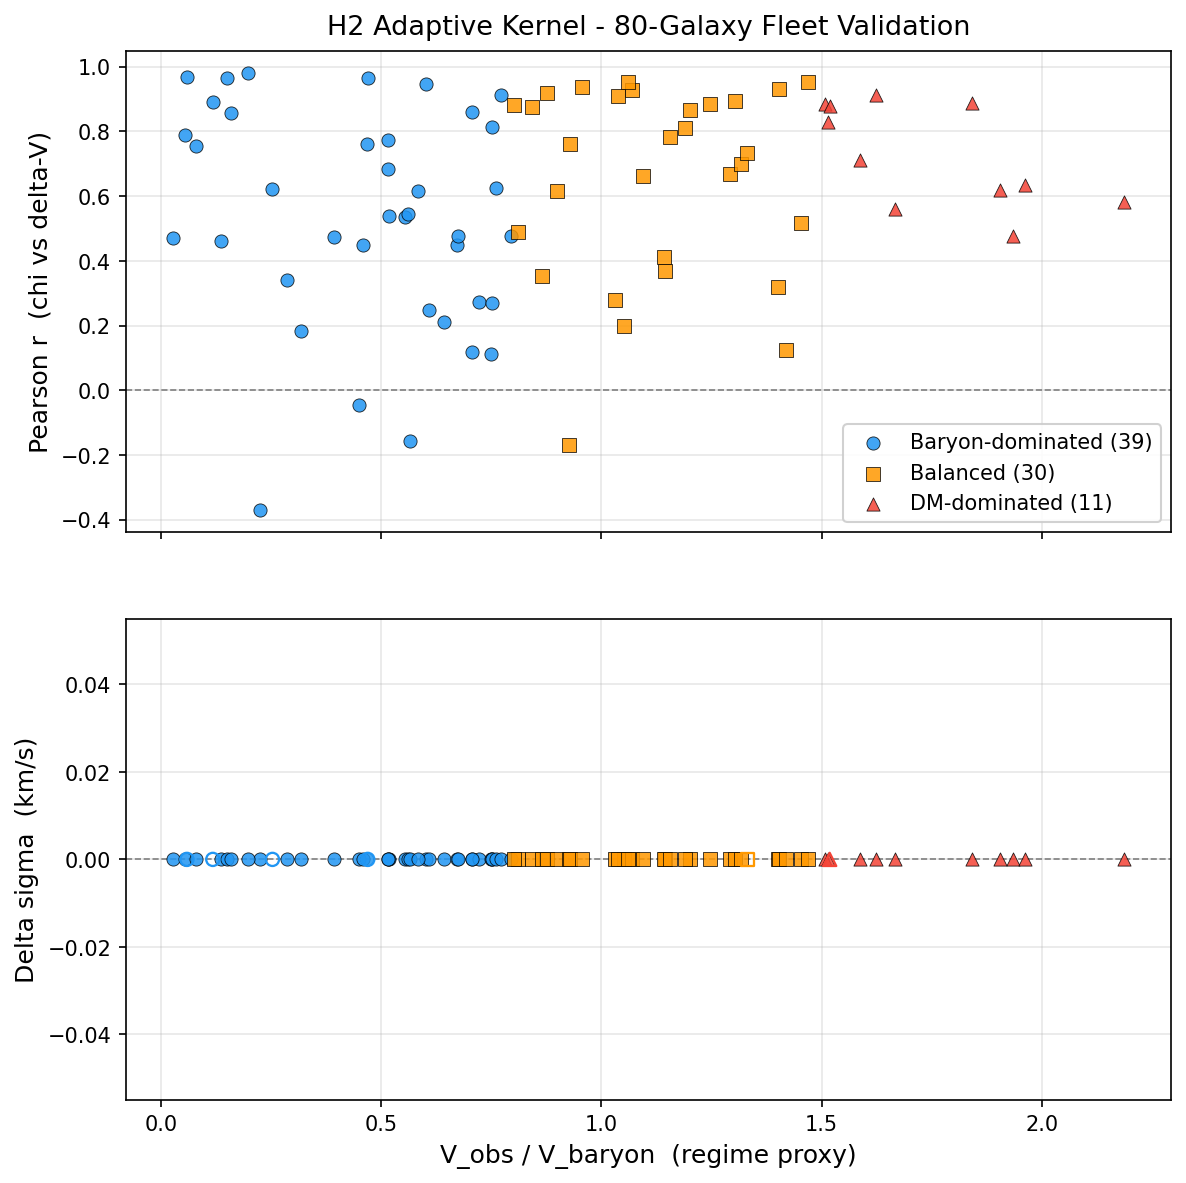
\includegraphics[width=\columnwidth]{regime_trends_80galaxy.png}
	\caption{Diagnostic metrics across dynamical regimes for the 80-galaxy
	sample. Top: Pearson correlation $r_{\mathrm{p}}$ between $\chi$ and
	$\Delta V$. Bottom: Change in scatter $\Delta\sigma\,(\mathrm{km\,s^{-1}})$.
	For 74 measured galaxies, $\Delta\sigma \approx 0\,\mathrm{km\,s^{-1}}$;
	6 galaxies with insufficient inner-region coverage are shown as open
	symbols. Correlation strength varies systematically with $\Vobs/V_b$
	across all three dynamical regimes.}
	\label{fig:regimes}
\end{figure}
\subsection{Magnitude scaling}

The maximum absolute velocity correction scales monotonically with regime:
\begin{itemize}
	\item Baryon-dominated: max$|\Delta V| \leq 0.43$ km s$^{-1}$
	\item Balanced: max$|\Delta V| \approx 0.15$--$0.40$ km s$^{-1}$
	\item Dark-matter-dominated: max$|\Delta V| \approx 2.5$ km s$^{-1}$
\end{itemize}
These corrections, while coherent with the adaptive mechanism, remain 
1--2 orders of magnitude below typical rotation curve residuals 
($\sim$10--50 km s$^{-1}$) and observational uncertainties.

\subsection{Geometric floor identification}

Across the 80-galaxy validation sample, the empirical operating floor remains
fixed at $L_{\mathrm{eff,min}} \approx L_0/3 = 66.67$ kpc, independent of
regime, morphology, or $\chi$ spatial pattern. Many systems reach this floor
directly, while others approach it asymptotically ($L_{\mathrm{eff,min}}$
range: 66.67 to 96.95 kpc), an operational limit within the present implementation.
This floor reflects the realized $\chi$-field range and taper constraints
of the adaptive response under fixed $L_0 = 200$ kpc, and defines a
structural boundary within the validated sample.
\begin{figure}
	\includegraphics[width=\columnwidth]{leff_overlay_80galaxy.png}
	\caption{Adaptive kernel scale $L_{\mathrm{eff}}(r)$ for all 80 galaxies
		(colored by $\Vobs/V_b$ ratio). All profiles reach or approach the
		empirical operating floor $L_0/3 = 66.67$ kpc (dashed horizontal line)
		in high-stiffness inner regions, independent of regime classification
		($L_{\mathrm{eff,min}}$ range: 66.67--96.95 kpc).}
	\label{fig:leff}
\end{figure}
\begin{table}[t]
	\caption{Summary statistics for the 80-galaxy H2 validation sample.}
	\label{tab:results}
	\centering
	\begin{tabular}{lc}
		\hline\hline
		Parameter & Value \\
		\hline
		Total galaxies & 80 \\
		Baryon-dominated ($\Vobs/V_b < 0.8$) & 39 \\
		Balanced ($0.8 \leq \Vobs/V_b < 1.5$) & 30 \\
		DM-dominated ($\Vobs/V_b \geq 1.5$) & 11 \\
		\hline
		$\Vobs/V_b$ range & $0.027$--$2.187$ \\
		Pearson $r$ range & $-0.371$--$+0.981$ \\
		\hline
		$\Delta\sigma \approx 0\,\mathrm{km\,s^{-1}}$ (measured) & 74 \\
		$\Delta\sigma = \mathrm{N/A}$ (inner coverage) & 6 \\
		Diagnostic protocol violations & 0 \\
		\hline
		$L_{\mathrm{eff}}$ floor (fleet-wide) & 66.67 kpc \\
		$L_{\mathrm{eff,min}}$ range & 66.67--96.95 kpc \\
		\hline
	\end{tabular}
	\tablefoot{$V_{\mathrm{obs}}/V_b$: observational velocity ratio used as a
		proxy for dynamical regime, computed as the ratio of peak velocity
		amplitudes of each component across the galactic radial profile.
		$\Delta\sigma$: change in inner scatter relative
		to H1 baseline. For all 74 measurable galaxies, $\Delta\sigma$ is consistent with zero within floating-point tolerance $(|\Delta\sigma| < 10^{-12}~\mathrm{km\,s^{-1}})$. The 6 N/A cases arise
		from data geometry (insufficient inner radial coverage) rather than
		model failure. Complete per-galaxy results are provided in the
		archived repository as \texttt{fleet\_summary\_80galaxy.csv}.}
\end{table}	
	%==============================================================================
	\section{Discussion}
	%==============================================================================
	
	\subsection{Quadrature suppression mechanism}
	
	The invariance of the inner scatter statistic ($\Delta\sigma \approx 0\,\mathrm{km\,s^{-1}}$
	for all measurable systems) indicates that bounded local scale modulation
	does not alter the inner-region scatter of the model under quadrature
	combination (Eq.~\ref{eq:vtot}). This behavior arises directly from the
	mathematical structure of the total velocity.
	This result also clarifies the trajectory from H1.5 to H2. The H1.5 diagnostics identified structured
	local mismatch under frozen canonical constraints, while H2 tests whether bounded local scale adaptation
	can remove that mismatch without altering the baseline implementation. The present 80-galaxy analysis
	shows that this form of bounded local adaptation does not alter the inner scatter metric within the
	validated subset.
	In baryon-dominated inner regions, the Newtonian component $V_{\mathrm{b}}$ 
	contributes the dominant term to 
	$V_{\mathrm{tot}} = \sqrt{V_{\mathrm{b}}^2 + V_{\mathrm{NL}}^2}$. 
	In this regime, variations in $V_{\mathrm{NL}}$ induced by scale contraction 
	produce second-order corrections to the total velocity. The sensitivity of 
	$V_{\mathrm{tot}}$ to changes in $L_{\mathrm{eff}}$ scales approximately as
\begin{equation}
	\frac{\partial V_{\mathrm{tot}}}{\partial V_{\mathrm{NL}}}
	=
	\frac{V_{\mathrm{NL}}}
	{\sqrt{V_b^2 + V_{\mathrm{NL}}^2}}
	\label{eq:vtot_derivative}
\end{equation}
	When $V_{\mathrm{b}} \gg V_{\mathrm{NL}}$, this sensitivity approaches zero,
	effectively suppressing the impact of adaptive kernel modulation on the total
	velocity profile. Consequently, even strong $\chi$--$\Delta V$ correlations
	(e.g., $r_{\mathrm{p}} = +0.95$ in IC2574, $r_{\mathrm{p}} = +0.981$ in
	UGC07577) do not translate into measurable reductions in the total residual
	amplitude.
	Within the present validation sample, the suppression identified in 
	Eq.~\ref{eq:vtot_derivative} is most effective when the nonlocal 
	contribution remains subdominant relative to the baryonic term in 
	the inner regions. The fixed scale $L_0 = 200$ kpc should therefore 
	be interpreted here as a phenomenological coupling scale of the 
	implementation rather than as a localized interaction range tied 
	to optical disk size.
	This relation shows that perturbations in the nonlocal component are 
	suppressed when $V_{\mathrm{NL}} \ll V_b$, explaining why adaptive 
	scale modulation produces limited changes in the total velocity.
	\begin{figure}
		\includegraphics[width=\columnwidth]{rc_comparison_NGC3198.pdf}
		\caption{Rotation-curve comparison for NGC3198 (balanced regime,
			$V_{\mathrm{obs}}/V_b = 1.42$). Observed data (points), H1 baseline
			(solid line), and H2 adaptive model (dashed line). Despite inner
			$L_{\mathrm{eff}}$ contraction toward the empirical operating floor,
			quadrature suppression limits the impact on the total velocity profile.}
		\label{fig:rc_example}
	\end{figure}
	This suppression arises from the quadrature structure itself, rather than 
	from numerical instability or insufficient correlation strength. The adaptive 
	mechanism operates coherently within its allowed bounds, but the mathematical 
	coupling limits its leverage in regions where one component dominates.
	
	\subsection{Role of the empirical operating floor}

	The adaptive response saturates at an empirical operating floor
	$L_{\mathrm{eff}} \approx L_0/3$, which is reached systematically in
	high-stiffness regions across the sample. This floor emerges from the
	realized $\chi$-field range and taper constraints rather than from the
	hard minimum of the discretized basis (which extends to $0.05\,L_0$),
	and it prevents further contraction of the nonlocal kernel in practice.

	The fact that the adaptive mechanism saturates at this floor without
	modifying the inner scatter metric indicates that further reduction of
	inner residuals cannot be achieved through scale contraction alone while
	$L_0$ and $\mu$ remain fixed. The empirical floor therefore represents an operational
	boundary of the present framework: within fixed global parameters, local
	scale adaptation is insufficient to modify the overall statistical
	dispersion of the rotation curve residuals.
	
	\subsection{Assessment of achieved and unachieved objectives}
	
	The H2 extension shows:
	\begin{itemize}
		\item coherent response of the kernel scale to baryonic gradient structure,
		\item regime-dependent modulation of $V_{\mathrm{NL}}$,
		\item preservation of outer-regime stability,
		\item strict numerical neutrality in the inner scatter metric.
	\end{itemize}
	
	However, the adaptive extension does not:
	\begin{itemize}
		\item reduce the inner-region scatter metric,
		\item eliminate inner-region overshoot,
		\item introduce measurable improvement in rotation-curve fits.
	\end{itemize}
	
	These findings indicate that the residual structure observed in H1 is not 
	attributable solely to the absence of local scale modulation. Instead, it 
	appears to be a structural property of the isotropic kernel formulation 
	under fixed global parameters.
	
	\subsection{Interpretation of scatter neutrality}

	The consistent result of $\Delta\sigma \approx 0\,\mathrm{km\,s^{-1}}$
	for all galaxies with sufficient inner-region coverage, together with
	6 undefined inner-coverage cases, warrants careful interpretation.
	Several independent lines of evidence support the interpretation that this is a systematic pattern rather than a numerical artifact.

	\textbf{(1) Active kernel response.} Pearson correlations range from
	$-0.371$ to $+0.981$, indicating the adaptive kernel responds
	differently to each galaxy's local baryonic structure. The modulation
	field is not dormant.

	\textbf{(2) Independence from baseline quality.} Systems with poor H1
	baseline fits (MAFE $> 0.9$, including NGC2403 with MAFE $= 1.67$ and
	NGC0024 with MAFE $= 1.57$) maintain scatter neutrality identically to
	those with excellent fits ($\mathrm{MAFE} < 0.1$), confirming that the
	result is not sensitive to H1 fit quality across the tested range.

	\textbf{(3) Fleet-wide empirical floor.} All 80 galaxies reach or
	approach $L_{\mathrm{eff,min}} \approx L_0/3 = 66.67$ kpc, confirming that
	the adaptive mechanism reaches its empirical operating floor across the
	full range of dynamical regimes.

	\textbf{(4) Sample breadth.} 80 galaxies spanning
	$\Vobs/V_b = 0.027$ to $2.187$ constitute a broader validation sample
	across morphological types, surface brightness regimes, and baryonic
	fractions.

	The observed pattern --- active local adaptation with invariant scatter
	--- could reflect: (a) a structural constraint arising from the
	quadrature velocity coupling, (b) saturation at the geometric floor
	preventing further kernel contraction, or (c) limited sensitivity of
	the adopted scatter metric to sub-km\,s$^{-1}$ local adjustments.
	Distinguishing these interpretations requires further investigation
	beyond the scope of this diagnostic study.

	\subsection{Implications for bounded nonlocal models}
	
	The present analysis defines a constraint on state-driven adaptive nonlocal 
	kernels operating under quadrature combination. When the effective
	contribution of the nonlocal term remains subdominant, bounded local
	modulation does not alter the inner scatter statistic.
	
	This result provides a diagnostic benchmark for future extensions of nonlocal
	modeling frameworks. Within the present framework, any modification intended to reduce the
	inner scatter metric must overcome the suppression mechanism identified here, either
	through alternative coupling structures, modified kernel functional forms,
	or adjustments to global baseline parameters.
	
	The H2 results therefore serve as a controlled null-response baseline for 
	evaluating more complex formulations. The framework establishes reproducible 
	boundary conditions that can inform the design space of adaptive gravitational 
	models.
%==============================================================================
\section{Conclusions}
%==============================================================================

We have characterized the structural and statistical limits of a bounded
adaptive nonlocal kernel framework (H2) for modeling galaxy rotation curves.
By extending a frozen baseline configuration with a state-driven
scale-modulation field $\chi(r)$, we isolated the impact of local baryonic
structure on the effective gravitational response. Diagnostic evaluation
across an 80-galaxy validation sample from the SPARC database reveals three
principal findings.

First, the adaptive mechanism demonstrates coherent regime-dependent coupling
between the stiffness field $\chi(r)$ and local velocity adjustments. The
systematic variation in Pearson correlation from $r_{\mathrm{p}} = -0.371$
to $+0.981$ across dynamical regimes indicates that scale modulation
operates consistently within the tested implementation.

Second, the empirical operating floor $L_{\mathrm{eff}} \approx L_0/3$ is
reached or approached in high-stiffness regions across all 80 galaxies
($L_{\mathrm{eff,min}}$ range: 66.67--96.95 kpc). This floor establishes
an operational boundary for local adaptation under fixed global scaling and
prevents further contraction of the nonlocal kernel within the validated sample.

Third, and most significantly, $\Delta\sigma$ is consistent with zero for
all galaxies with sufficient inner-region coverage; 6 systems are undefined
due to inner-coverage limitations. Across all 80 galaxies, no measurable departure from inner-scatter neutrality was found beyond floating-point tolerance. Quadrature coupling, together with the empirical operating floor and the bounded adaptive range,
suppresses the influence of local scale contraction on the total velocity, and local state-driven deformation alone is insufficient to modify the inner-region scatter metric.

These findings indicate that the residual structure observed in the frozen
baseline cannot be removed solely by introducing bounded local scale
variability. Within the bounded adaptive implementation examined here,
modifications that aim to alter the inner scatter metric must overcome
the suppression mechanism identified in this study.

The H2 implementation is publicly archived and fully reproducible. It
provides a reproducible diagnostic benchmark for bounded adaptive
nonlocal kernel models.

%==============================================================================
\begin{acknowledgements}
	This research made use of rotation curve data from the Spitzer Photometry
	and Accurate Rotation Curves (SPARC) database \citep{lelli2016}. We thank
	the developers of NumPy \citep{numpy2020}, SciPy \citep{scipy2020},
	Matplotlib \citep{matplotlib2007}, and pandas \citep{pandas2010} for
	providing the scientific Python ecosystem.
	The author used large language models for limited technical assistance in
	code debugging, Python scripting, implementation support, LaTeX editing,
	and language polishing. All scientific design, data analysis,
	interpretation, and conclusions are the sole responsibility of the author.
\end{acknowledgements}

%==============================================================================

\section*{Data availability}

The complete H2 framework code, diagnostic pipeline, and 80-galaxy
validation results, including \texttt{fleet\_summary\_80galaxy.csv} and
associated figures from \texttt{fleet\_expansion\_80galaxy/}, are publicly
archived at \url{https://doi.org/10.5281/zenodo.18911959} under an MIT
license. The development repository for the project is available at
\url{https://github.com/VitorFigueiredoResearch/H2-Adaptive-Kernel-Framework-for-Galaxy-Rotation-Curves}.
Rotation curve data from the SPARC database \citep{lelli2016} are
available at \url{http://astroweb.cwru.edu/SPARC/}. All results presented
in this paper are reproducible using the archived code together with the
publicly available SPARC data.

\appendix
\section{H1 Baseline Framework: Formalism and Implementation}
\label{app:h1}

The H2 adaptive framework builds upon the H1 frozen baseline \citep{figueiredo2024_h1, figueiredo2024_h1p5}. To ensure reproducibility and self-containment, we provide both (1) the formal H1 equations as presented in the manuscript, and (2) the specific numerical implementation used in this work, archived publicly at \href{https://doi.org/10.5281/zenodo.18793233}{https://doi.org/10.5281/zenodo.18793233}.

\subsection{H1 formalism (from manuscript)}

The H1 effective potential is decomposed as:
\begin{equation}
	\Phi_{\mathrm{eff}}(\mathbf{r}) = \Phi_{\mathrm{b}}(\mathbf{r}) + \Phi_{\mathrm{K}}(\mathbf{r}),
	\label{eq:phi_eff}
\end{equation}
where $\Phi_{\mathrm{b}}$ is the Newtonian baryonic potential and $\Phi_{\mathrm{K}}$ is the kernel-induced nonlocal contribution defined by:
\begin{equation}
	\Phi_{\mathrm{K}}(\mathbf{r}) = \mu G \int \rho_{\mathrm{b}}(\mathbf{r}') \, U(|\mathbf{r} - \mathbf{r}'|; L) \, d^3r',
	\label{eq:convolution}
\end{equation}
where $\mu$ is a dimensionless coupling parameter, $L$ is the kernel characteristic scale, and $U(r;L)$ is an isotropic radial kernel function normalized such that $\int U(r;L) d^3r = 1/L$.

The circular velocity is derived from the radial gradient of the effective potential:
\begin{equation}
	V^2_{\mathrm{tot}}(R) = R\, \frac{\partial \Phi_{\mathrm{eff}}}{\partial R}\Bigg|_{z=0}.
	\label{eq:v_gradient}
\end{equation}

For numerical stability, this is implemented as a quadrature decomposition:
\begin{equation}
	V^2_{\mathrm{tot}}(R) = V^2_{\mathrm{b}}(R) + V^2_{\mathrm{K}}(R),
	\label{eq:v_quadrature}
\end{equation}
where $V_{\mathrm{b}}$ is the Newtonian baryonic contribution and $V_{\mathrm{K}}$ is the kernel-induced contribution. This decomposition is a computational identity and does not imply physical independence \citep{figueiredo2024_h1}.

The H1 framework explores a fixed parameter grid:
\begin{equation}
	L \in [20, 200]\,\mathrm{kpc}, \quad \mu \in [1, 500],
	\label{eq:param_grid}
\end{equation}
sampled logarithmically to identify optimal $(L, \mu)$ pairs for each galaxy.

\subsection{Numerical implementation specification}

To ensure exact reproducibility of the H2 diagnostic pipeline, we specify the numerical implementation of H1 used in this work, publicly archived with DOI \href{https://doi.org/10.5281/zenodo.18793233}{10.5281/zenodo.18793233}.

\subsubsection{Kernel functional form}

While the H1 manuscript defines the kernel $U(r;L)$ via its normalization and asymptotic properties, the specific analytic form implemented in the diagnostic pipeline is a regularized logarithmic kernel:\footnote{This implementation corresponds to the kernel architecture archived in the project repository and referred to internally in the development repository as the hybrid kernel.}
\begin{equation}
	U(r; L) = \frac{1}{2} \ln\left(1 + \frac{r^2_{\mathrm{safe}}}{L^2}\right),
	\label{eq:kernel_implementation}
\end{equation}
where $r_{\mathrm{safe}} = \sqrt{r^2 + \epsilon^2}$ with $\epsilon = 0.01\,L$ prevents singularity at $r = 0$. This functional form is consistent with the asymptotic properties described in H1 while providing numerical stability at small radii.

A finite-support taper is applied:
\begin{equation}
	T(r) = 
	\begin{cases}
		1, & r \le L \\
		\exp\left[-\left(\frac{r - L}{\Delta}\right)^2\right], & r > L,
	\end{cases}
	\label{eq:taper}
\end{equation}
with $\Delta = L$, truncating the kernel at $R_{\mathrm{cut}} = 6L$.

\subsubsection{Amplitude calibration}

Following validation diagnostics performed in H1.5, a global amplitude correction factor $\beta = 1.15$ was identified as necessary to account for finite-grid sampling effects and the discrete vertical disk prescription. This constant is applied uniformly across all galaxies in the archived implementation:
\begin{equation}
	\hat{\Phi}_{\mathrm{K}}(\mathbf{k}) = \mu \beta G\, \hat{\rho}_{\mathrm{b}}(\mathbf{k})\, \hat{U}(\mathbf{k}),
	\label{eq:fourier_beta}
\end{equation}
where the convolution is evaluated in Fourier space for computational efficiency.

\subsection{Eighty-galaxy H2 baseline parameters}

All 80 galaxies in the H2 validation set share identical H1 frozen parameters in the archived implementation:
\begin{equation}
	L_0 = 200\,\mathrm{kpc}, \quad \mu = 10, \quad \beta = 1.15.
	\label{eq:h2_baseline_params}
\end{equation}

These values define the compatibility condition for H2 adaptive convolution under taper constraints. Galaxies whose H1 best-fit parameters differ from this canonical baseline require recalibration of the adaptive response and were excluded to maintain the homogeneity of the present diagnostic study (see Section 3.1).

Table~A.1 presents representative H1 baseline rotation-curve metrics for the original 30-galaxy validation subset used during the staged construction of the 80-galaxy H2 sample.

\begin{table}[p]
	\caption{Representative H1 baseline rotation-curve metrics for the original 30-galaxy validation subset of the 80-galaxy H2 sample. All values computed from the archived H1 frozen-parameter pipeline with $(L_0, \mu, \beta) = (200\,\mathrm{kpc}, 10, 1.15)$.}
	\label{tab:h1_baseline}
	\centering
	\small
	\begin{tabular}{lcc}
		\hline\hline
		Galaxy & MAFE$_{\mathrm{H1}}$ & $V_{\mathrm{kernel}}/V_{\mathrm{bar}}$ \\
		\hline
		NGC~6946  & 0.139 & 1.11 \\
		NGC~2903  & 0.227 & 1.73 \\
		NGC~5585  & 0.409 & 0.95 \\
		NGC~0891  & 0.120 & 0.92 \\
		NGC~7793  & 0.380 & 0.73 \\
		NGC~2998  & 0.141 & 1.23 \\
		NGC~0024  & 1.569 & 2.94 \\
		IC~2574   & 0.224 & 0.81 \\
		NGC~3893  & 0.188 & 1.42 \\
		DDO~161   & 0.478 & 1.13 \\
		NGC~3769  & 0.759 & 2.38 \\
		NGC~3726  & 0.510 & 2.03 \\
		NGC~1003  & 0.277 & 1.29 \\
		NGC~3198  & 1.380 & 2.40 \\
		NGC~5033  & 0.304 & 2.37 \\
		NGC~3953  & 0.088 & 1.21 \\
		NGC~3521  & 0.429 & 1.51 \\
		NGC~3992  & 0.258 & 2.57 \\
		UGC~03580 & 1.398 & 2.04 \\
		UGC~06983 & 0.124 & 1.43 \\
		NGC~5055  & 0.387 & 2.26 \\
		UGC~07608 & 0.190 & 1.16 \\
		UGC~02259 & 0.226 & 2.14 \\
		NGC~4100  & 0.127 & 1.90 \\
		KK~98-251 & 0.217 & 1.15 \\
		UGC~05716 & 0.246 & 1.84 \\
		F~571-8   & 0.338 & 2.12 \\
		NGC~6503  & 0.226 & 2.75 \\
		NGC~2403  & 1.673 & 3.17 \\
		NGC~2955  & 0.175 & 2.25 \\
		\hline
	\end{tabular}
	\tablefoot{Mean absolute fractional error (MAFE) quantifies rotation curve fit quality. The ratio $V_K/V_b$ reported here is an H1 baseline diagnostic quantity and
		is distinct from the $V_{\mathrm{obs}}/V_b$ regime proxy used in the main H2 analysis. This table shows the original 30-galaxy validation subset. The complete 80-galaxy baseline parameters are archived as \texttt{fleet\_summary\_80galaxy.csv}.}
\end{table}

The H2 adaptive framework retains this H1 baseline in its entirety across all 80 galaxies, introducing only local kernel scale modulation $L_{\mathrm{eff}}(r)$ as a diagnostic modification while holding $(L_0, \mu, \beta)$ fixed. All H2 results are differential comparisons against this frozen baseline.
%==============================================================================
% BIBLIOGRAPHY
%==============================================================================
\bibliographystyle{aa}
\bibliography{references}

\end{document}


